\documentclass[12pt, a4paper]{report}
\usepackage[spanish]{babel}
\usepackage{graphicx}
\usepackage{times}
\usepackage{geometry}
\usepackage{csquotes}
\usepackage{parskip}
\usepackage{fancyhdr}
\usepackage{lipsum}
\usepackage{graphicx}
\usepackage{hyperref}
\usepackage{longtable}
\usepackage{pgfplots}
\pgfplotsset{compat=1.18}
\usepackage[style = apa, backend = biber]{biblatex}
\usepackage{setspace}
\usepackage{array}
\usepackage{float}
\usepackage{booktabs}
\usepackage{multicol}
\usepackage{esdiff}
\usepackage{titlesec}
\usepackage{titletoc}
\usepackage{listings} 
\renewcommand{\thechapter}{\Roman{chapter}}
\renewcommand{\thesection}{\arabic{chapter}.\arabic{section}}
\renewcommand{\thesubsection}{\arabic{chapter}.\arabic{section}.\arabic{subsection}}
\renewcommand{\thetable}{\arabic{chapter}.\arabic{table}}
\renewcommand{\thefigure}{\arabic{chapter}.\arabic{figure}}
\renewcommand{\theequation}{\arabic{chapter}.\arabic{equation}}
\usepackage{caption}
\captionsetup[figure]{labelformat=simple, labelsep=none, labelfont={bf}, textfont={it}, singlelinecheck=off}
\renewcommand{\figurename}{Figura}
\DeclareCaptionFormat{custom}{#1#2\\#3} 
\captionsetup[figure]{format=custom}
\captionsetup[table] {labelformat=simple, labelsep=none, labelfont={bf}, textfont={it}, singlelinecheck=off}
\renewcommand{\tablename}{Tabla}
\captionsetup[table]{format=custom}
\newcommand\blankpage{%
    \null
    \thispagestyle{empty}%
    \addtocounter{page}{-1}%
    \newpage}


% Recursos bibliográficos
\addbibresource{ref.bib}


% Formato de página
\geometry{a4paper, left=3.5cm,right=2.54cm,top=2.54cm,bottom=2.54cm}
\setlength{\parindent}{2em}
\pagestyle{fancy}
\fancyhf{} % clear all header and footer fields
\renewcommand{\headrulewidth}{0pt} % no line in header area
\fancyfoot[R]{\thepage} % page number in the right footer
\fancypagestyle{plain}{%
  \fancyhf{} % clear all header and footer fields
  \fancyfoot[R]{\thepage} % page number in the right footer
}

% Documento

\begin{document}
\titleformat{\chapter}[block]
  {\centering\bfseries\Large} % Format: centered, bold, large size
  {CAPÍTULO \thechapter:} % Chapter label
  {5pt} % Space between label and title
  {\MakeUppercase} % Title formatting
\titlespacing*{\chapter}{0pt}{-30pt}{20pt} % Adjust spacing: {left}{before}{after}
\titleformat{\section}{\normalfont\bfseries}{\thesection}{1em}{}
\titleformat{\subsection}{\normalfont\bfseries}{\thesubsection}{1em}{}

%%% CONTENIDO %%%%%%%%%%
\pagenumbering{roman}
\renewcommand{\thepage}{\expandafter{\romannumeral\value{page}}}
\begin{titlepage}
    \centering
    {\scshape\large Universidad de Málaga \par}
    \vspace{0.3cm}
    {\scshape\large Programación Segura \par}
     \vspace{0.3cm}
     
    
\includegraphics[width=0.5\textwidth]{frontmatter/simple-black-pj-logo-vector-260nw-1799911108-removebg-preview.png}\\[0.3cm]
    {\LARGE\bfseries Práctica 2: buffer overflows y strings \par}
    \vspace{0.3cm}
     {\scshape\large Ciberseguridad e Inteligencia Artificial \par}
    \vspace{0.3cm}
    
    {\Large\bfseries Pablo Jesús Delgado Muñoz \par}
    \vspace{0.5cm}
    \vfill
    
    
    {\large Octubre de 2024\par}
    \vspace{1cm}


\let\cleardoublepage\clearpage
\tableofcontents
\let\cleardoublepage\clearpage

\end{titlepage}


\renewcommand{\baselinestretch}{1.5} 
\pagenumbering{arabic}
%\chapter*{INTRODUCCIÓN}
\addcontentsline{toc}{section}{\textbf{INTRODUCCIÓN}}

\noindent
En esta práctica, nos adentraremos en el estudio y solución de un problema crítico en la programación: el desbordamiento de búfer (buffer overflow). Este fenómeno ocurre cuando un programa escribe más datos en un área de memoria de lo que estaba previsto, lo que puede causar fallos graves, desde comportamientos inesperados hasta vulnerabilidades de seguridad que los atacantes pueden explotar. Durante el desarrollo de esta práctica, aprenderemos a identificar este tipo de errores en el código y a corregirlos de manera eficiente, utilizando diversas herramientas de desarrollo y depuración.
\vspace{0.3cm}
\\
El propósito de esta práctica es, no solo entender qué es un desbordamiento de búfer, sino también adquirir las habilidades necesarias para detectarlo en código real. Herramientas como Valgrind serán clave para analizar la memoria utilizada por el programa y detectar problemas. Como editor de texto usaré Kate debido a preferencia personal y exploraremos otras herramientas útiles que facilitan el proceso de depuración.
\vspace{0.3cm}
\\
Cabe destacar que el ingeniero, por naturaleza, busca optimizar sus procesos y resultados, minimizando el tiempo de trabajo y maximizando la eficiencia. A lo largo de esta práctica, descubriremos varias estrategias y herramientas que nos permitirán cumplir con este objetivo. Estas herramientas no solo mejorarán nuestro flujo de trabajo, sino que también permitirán que el código sea más robusto, seguro y eficiente. \par

\chapter{Buffer Overflow}

\section{Definición y explicación}
\noindent El \textbf{buffer overflow} o desbordamiento de búfer es un fenómeno que ocurre cuando un programa intenta almacenar más datos en un bloque de memoria (\textit{buffer}) del que este puede contener. Los búferes son segmentos de memoria reservados específicamente para almacenar datos temporalmente. Estos datos pueden variar ampliamente, desde entradas del usuario, datos recibidos de un archivo, hasta paquetes de información que forman parte de comunicaciones en red. Sin embargo, cuando los datos que se intentan almacenar sobrepasan la capacidad asignada al búfer, se produce un desbordamiento. En esta situación, los datos excedentes se expanden hacia otras zonas de la memoria, sobrescribiendo potencialmente información crítica que el programa no tenía intención de modificar, lo cual puede alterar su funcionamiento.

\vspace{0.3cm}
\noindent Este tipo de vulnerabilidad es particularmente común en lenguajes de programación como \texttt{C} o \texttt{C++}, donde la gestión de la memoria no es controlada de manera automática por el lenguaje. En estos lenguajes, la memoria asignada a cada variable es administrada manualmente por el programador o, de manera predeterminada, sin verificación de límites. Cuando se intenta escribir más información en un búfer del que este puede albergar, los datos adicionales pueden sobrescribir variables adyacentes, estructuras de control del programa, o incluso direcciones de retorno en la pila de memoria. En el peor de los casos, esto puede hacer que el programa falle de manera catastrófica, se comporte de manera errática, o, en los casos más graves, ejecute código malicioso que haya sido inyectado por un atacante. Esto último es particularmente peligroso cuando el desbordamiento afecta regiones de memoria sensibles o protegidas del sistema, que el programa no tiene autorización para modificar.

\vspace{0.3cm}
\noindent Los buffer overflows no siempre son fáciles de detectar, ya que pueden no causar problemas visibles durante la ejecución normal del software, y es posible que pasen desapercibidos por largos periodos de tiempo. Sin embargo, la ausencia de síntomas evidentes no implica que el problema sea menor o inofensivo. Un desbordamiento puede generar fallos importantes en el programa y en la integridad de los datos, especialmente en aplicaciones que manejan grandes volúmenes de datos o que se ejecutan durante largos periodos de tiempo. Estos fallos pueden comprometer la fiabilidad, seguridad y usabilidad del software.

\newpage
\subsection{Por qué es un problema grave}
\noindent 
El \textbf{desbordamiento de búfer} es considerado una vulnerabilidad grave en el ámbito de la seguridad informática, y no necesariamente debe ser explotado por un atacante para que represente un riesgo significativo. A menudo, los desbordamientos de búfer pueden estar presentes en un sistema durante mucho tiempo sin ser detectados, y sin provocar consecuencias inmediatas. Esto no significa que su presencia sea inofensiva; de hecho, un desbordamiento de búfer puede causar problemas muy serios en el funcionamiento de un programa en diversas formas.

\vspace{0.3cm}
\noindent Un aspecto importante a tener en cuenta es que un desbordamiento de búfer puede corromper los datos almacenados en áreas de la memoria que son esenciales para el funcionamiento adecuado del software. Este tipo de corrupción de datos puede llevar a \textbf{fallos aleatorios} en el programa, los cuales son notoriamente difíciles de depurar. Estos fallos suelen manifestarse solo en circunstancias específicas, como cuando se introducen valores de entrada que exceden el tamaño permitido por el búfer. Esto da lugar a lo que se conoce como \textbf{errores intermitentes}, que son complicados de diagnosticar debido a que no se producen de forma constante, y no siempre es sencillo reproducir las condiciones que los desencadenan.

\vspace{0.3cm}
\noindent Un desbordamiento de búfer también puede \textbf{interrumpir el flujo de ejecución del programa}, provocando bloqueos, pérdida de datos o respuestas inesperadas. Esto es problemático no solo porque afecta la experiencia del usuario, sino porque compromete la estabilidad general del sistema en el que el programa se está ejecutando. Un programa que falla ocasionalmente en ciertas circunstancias puede afectar a otros procesos y servicios que dependan de él, generando una \textbf{cascada de fallos} en otros componentes del sistema. Esto puede llevar a un colapso total en aplicaciones de misión crítica, donde la confiabilidad y la estabilidad son esenciales para el funcionamiento del sistema en su conjunto.

\vspace{0.3cm}
\noindent Más allá de los problemas de integridad de datos y estabilidad, el desbordamiento de búfer presenta un \textbf{riesgo significativo de seguridad}. En situaciones donde un atacante puede controlar los datos que se ingresan en un búfer, puede aprovechar el desbordamiento para modificar la memoria del sistema de forma deliberada metiendo shellcode. En algunos casos, el atacante podría alterar el flujo de ejecución del programa para ejecutar código arbitrario(shellcode), dándole la posibilidad de tomar el control total del sistema en el que el programa vulnerable se está ejecutando. Por esta razón, los desbordamientos de búfer son uno de los vectores de ataque más comunes en exploits y ataques de escalación de privilegios.

\vspace{0.3cm}

\chapter{DETECCIÓN DEL PROBLEMA}
\noindent En este capítulo vamos a adentrarnos en el análisis, detección y busca de soluciones para  el buffer overflow. Primero veremos una serie de herramientas muy útiles, los procesos realizados para detectar estas vulnerabilidades, impacto de estas mismas.

\section{Herramientas utlilizadas}
\noindent Para abrir, analizar y leer código, podemos utilizar una gran variedad de editores de texto y combinar estos con diferentes herramientas que facilitan el trabajo de desarrollo y depuración. Destacamos \textbf{Vim} , {\textbf{SublimeText}} o {\textbf{Kate}} como editores de texto.
\\\\
Para facilitar la depuración, emplearemos \textbf{Valgrind}, un conjunto de herramientas muy útil para encontrar errores de administración de memoria y subprocesamiento en código.
\\\\
Cuando recibimos código para revisar en busca de errores, muchas veces podemos encontrar que este no se encuentra correctamente indentado u organizado. Por lo tanto, para evitar cometer errores organizando el código por nosotros mismos, emplearemos \textbf{Indent}.

\section{Análisis código original}
\noindent Primero que nada vamos a abrir el código proporcionado por primera vez, usaremos Vim.  Nos movemos a la carpeta donde se encuentra en código y lo abrimos.
\\\\
 
\includegraphics[width=1\textwidth]{mainmatter/Fotos Codigo/1.png}
 \\\\
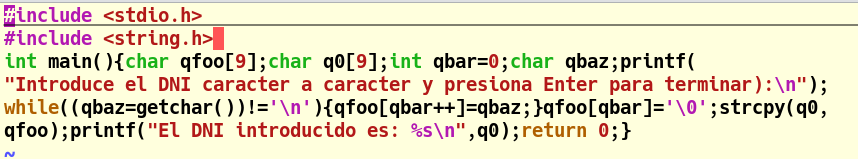
\includegraphics[width=1\textwidth]{mainmatter/Fotos Codigo/codigo sin indent.png}
\\\\
\noindent Podemos observer que el código no está totalmente ordenado, por lo tanto emplearemos el comando Indent para evitar errores y hacer de forma automática el indentado del código.
\\\\
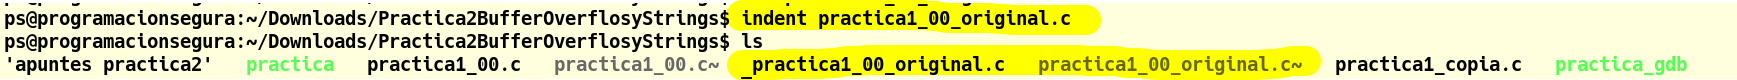
\includegraphics[width=1\textwidth]{mainmatter/Fotos Codigo/indent1.png}

\newpage 
\noindent Abrimos el código de nuevo y podemos ver que ya está correctamente formateado.
%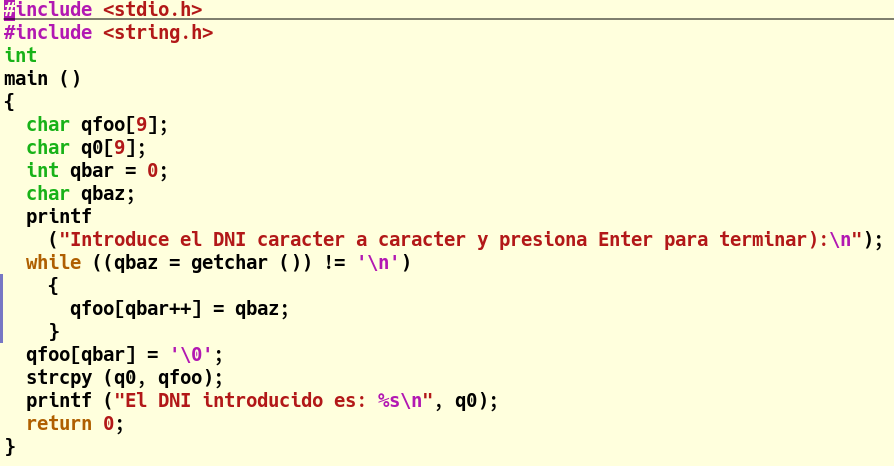
\includegraphics[width=1\textwidth]{mainmatter/Fotos Codigo/codigo formateado.png}
\\
\noindent Podemos ahora observar un fragmento de código en C que al parecer lee un DNI caracter a caracter, almacenándolo, y tras leer lo vuelve a imprimir.
\begin{verbatim}
#include <stdio.h>
#include <string.h>
int
main ()
{
  char qfoo[9]; //reservamos 9 caracteres en qfoo
  char q0[9]; //reservamos 9 caracteres en q0
  int qbar = 0; //inicializamos qbar a 0
  char qbaz;  //creamos variable qbaz de tipo caracter
  printf
    ("Introduce el DNI caracter a caracter y presiona 
    Enter para terminar):\n");
  while ((qbaz = getchar ()) != '\n') 
    //en qbaz guardamos lo que leemos y entramos al bucle            //mientras sea distinto de salto de línea
    {
      qfoo[qbar++] = qbaz; 
      //guardamos en cada iteración del while (donde qbar              //incrementa++), el caracter leído qbaz dentro de qfoo
    }
  qfoo[qbar] = '\0'; //ponemos el caracter nulo en la 
  //ultima posicion de qfoo (qbar)
  strcpy (q0, qfoo);  //hacemos strcpy de qfoo a q0, para                  //imprimir luego q0. OJO! STRCPY es insegura...
  printf ("El DNI introducido es: %s\n", q0);
  return 0;
}
\end{verbatim}

\noindent Primero crea un array qfoo de 9 caracteres,  q0[9], que es similar a qfoo y se crea un entero qbar inicializado en 0.
\\Ahora tras incializar los datos necesarios, el código imprime el mensaje que pide que se introduzca el DNI, y dentro del while se accederá a qfoo usando qbar como indice aumentando este uno a uno para así moverse dentro de qfoo. Asignará en cada posición el valor de qbaz, que es el caracter introducido en cada interación del bucle.
\\Ya por último se introduce el carácter nulo en qfoo y se usa strcpy para copiar el string de qfoo a q0, y se imprime q0 por pantalla.


\newpage
\section{Proceso de detección del problema}
\noindent Para detectar el problema vamos a ver si el problema "parece" hacer lo que debe:
\\Compilamos y ejecutamos: \\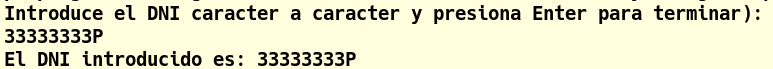
\includegraphics[width=1\textwidth]{mainmatter/Fotos Codigo/simple vista.png}
A simple vista, parece que el programa funciona correctamente, pero debemos tener en cuenta que cuando un programa entra para buscar problemas con él, ha pasado ciertas pruebas, por lo tanto, es normal que "aparentemente" funcione correctamemte. Vamos entonces a adentrarnos en materia y analizar el programa usando \textbf{Valgrind}.
\\
\vspace{0.3cm}
\noindent Primero compilamos el programa de nuevo pero con el flag -g para obtener trazas de debugging y poder usar valgrind.
\\
\includegraphics[width=1\textwidth]{mainmatter/Fotos Codigo/captura compilar debugging.png}
\\
Ejecutamos ahora el programa con valgrind...
\\
\textbf{El DNI introducido es: 888888888 }

==5378== HEAP SUMMARY: 
\\
==5378==     in use at exit: 0 bytes in 0 blocks 
\\
==5378==   total heap usage: 2 allocs, 2 frees, 2,048 bytes allocated 
\\
==5378== All heap blocks were freed -- no leaks are possible 
\\
==5378== ERROR SUMMARY: 1 errors from 1 contexts (suppressed: 0 from 0) 
\\
==5378== 1 errors in context 1 of 1: 
\\
==5378== Source and destination overlap in strcpy(0x1ffefffdd9, 0x1ffefffde2) 
\\
==5378==    at 0x484696F: strcpy (vg\_replace\_strmem.c:553) 
\\
==5378==    by 0x1091C6: main (practica1\_00.c:18) 
\\
\textbf{==5378== ERROR SUMMARY: 1 errors from 1 contexts (suppressed: 0 from 0)}
\vspace{0.3cm}
\\
\noindent Podemos observar como al introducir 9 caracteres el programa da error, mientras que si introducimos 8 caracteres no lo dará, por lo tanto se ha producido un buffer overflow.
\vspace{0.3cm}
\\
\textbf{El DNI introducido es: 8888888V }
\\
==5382== HEAP SUMMARY: 
\\
==5382==     in use at exit: 0 bytes in 0 blocks 
\\
==5382==   total heap usage: 2 allocs, 2 frees, 2,048 bytes allocated 
\\
==5382== All heap blocks were freed -- no leaks are possible 
\\
\textbf{==5382== ERROR SUMMARY: 0 errors from 0 contexts (suppressed: 0 from 0)}
\\
Los array qfoo y \verb|q0| están diseñados para almacenar un máximo de 9 caracteres. Sin embargo, cuando introduces un DNI de 9 dígitos, no queda espacio para el carácter nulo (\verb|\0|) que indica el final de una cadena en C. Al intentar copiar el contenido de \verb|qfoo| a \verb|q0| usando \verb|strcpy|, se produce un desbordamiento porque se intenta copiar un carácter más del que cabe en \verb|q0|.
\vspace{0.3cm}
\\
\textbf{¿Por qué no ocurre el error con 8 caracteres?}
\\
Cuando introduces 8 caracteres, el carácter nulo se almacena en la novena posición del arreglo, dejando espacio suficiente para ambos. Al utilizar \verb|strcpy|, se copia correctamente la cadena a \verb|q0| sin causar un desbordamiento.
\\
\newpage
\noindent Ahora vamos a hacer uso de la herramienta gdb para ver cómo se produce este buffer overflow:
\begin{verbatim}
ps@programacionsegura:$ gdb ./practica1\_debugging
(gdb) b 10 
Breakpoint 1 at 0x11b4: file practica1\_00\_original.c, line 17. 
(gdb) b 18 
Breakpoint 2 at 0x11c7: file practica1\_00\_original.c, line 18.
\end{verbatim}
\noindent Antes de causar el buffer overflow, vamos a ver dónde se escribe en memoria:
\begin{verbatim}
(gdb) x/64wx \$rsp 
0x7fffffffde40: 0x00000000 0x00000000 0x00000000 0x00000000 
0x7fffffffde50: 0x00000000 0x00000000 0x00000000 0x00000000 
0x7fffffffde60: 0x00000001 0x00000000 0xf7de424a 0x00007fff 

\end{verbatim}
\noindent Ahora cuando introducimos datos
\begin{verbatim}
Breakpoint 1, main () at practica1\_00\_original.c:17 
17        \textbf{strcpy} (q0, qfoo); 
(gdb) x/10wx \$rsp 
0x7fffffffde40: 0x00000000 0x00000000 0x00000000 0x00000000 
0x7fffffffde50: 0x39390000 0x39393939 0x0a003939 0x00000008 
    
\end{verbatim}
\noindent Saltamos a la linea 18 donde se hace strcpy...

\begin{verbatim}
Breakpoint 3, main () at practica1\_00\_original.c:18 
18   \textbf{printf} ("El DNI introducido es:, q0); 

(gdb) print qfoo 
\$2 = "99999999" OBSERVAMOS EL VALOR EN QFOO TRAS EL STRCPY

(gdb) x/64wx \$rsp 

0x7fffffffde40: 0x00000000 0x00000000 0x39393900 0x39393939 
0x7fffffffde50: 0x39390039 0x39393939 0x0a003939 0x00000008 
0x7fffffffde60: 0x00000001 0x00000000 0xf7de424a 0x00007fff 
 
\end{verbatim}
\noindent Si comparamos, podemos ver las posiciones de memoria en qfoo, pero ahora vamos a hacerlo pasándonos de datos a ver que ocurre:

\begin{verbatim}
Introduce el DNI caracter a caracter y presiona Enter para terminar): 
999999999999999999999999
99999999999999999999
99999999999999999999999999 

Breakpoint 1, main () at practica1\_00\_original.c:17 

17  \textbf{strcpy} (q0, qfoo); 

(gdb) x/10wx \$rsp 

0x7fffffffde40: 0x00000000 0x00000000 0x00000000 0x00000000 
0x7fffffffde50: 0x39390000 0x39393939 0x0a393939 0x00000074 
0x7fffffffde60: 0x00000001      0x00000000

\end{verbatim}

\noindent Aqui lo podemos observar antes del copy...

\begin{verbatim}
(gdb) x/10wx \$rsp 

0x7fffffffde40: 0x00000000 0x00000000 0x39393900 0x39393939 
0x7fffffffde50: 0x740a3939 0x39393900  0x0a393939 0x00000074 
0x7fffffffde60: 0x00000001 0x00000000 

(gdb) print qfoo 

\$1 = "\nt\n000999999"

\end{verbatim}
\noindent Podemos observar como lo que se encuentra en memoria ya comienza a fluctuar respecto de lo que deberíamos de ver si no hubiera problemas.
\newpage
\section{Ubicación y explicación del problema}
\noindent Ahora vamos a analizar el código para ver dónde se produce este buffer overflow. Como hemos visto al inicio del programa, se han reservado 9 posiciones en memoria para almacenar el string, pero claro, un DNI ocupa 9 posiciones, por lo tanto no se ha tenido en cuenta el carácter nulo,  que \verb|strcpy| usa para determinar el final de la cadena.
\vspace{0.3cm}
\\
\noindent Vamos a explicar los pasos que han llevado a este desbordamiento:
\begin{enumerate}
    \item \textbf{Almacenamiento del DNI en qfoo}
    \item \textbf{Uso de strcpy} / \textbf{no controlar el límite de lo que se lee}
    \item \textbf{Sobrescritura en memoria}
\end{enumerate}
Vamos a observar el array antes y después de usar strcpy:
\\
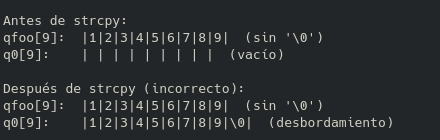
\includegraphics[width=0.75\textwidth]{mainmatter/Fotos Codigo/imagenantesdespuesstrcpy.png} 
\\
\section{Impacto del desbordamiento en la ejecución del programa}
\noindent Aunque el programa pueda seguir ejecutándose después de un desbordamiento de búfer, es fundamental comprender que esto no significa que el programa esté funcionando correctamente. Los efectos del desbordamiento pueden ser impredecibles y difíciles de detectar, pero siempre representan una amenaza para la seguridad y la estabilidad del programa.
\\
\newline Esto se debe básicamente a que en este programa, como es sencillo, no llegamos a hacer más cosas que imprimir únicamente el dni que hemos introducido, por lo tanto no hay mucha posibilidad de que este buffer overflow afecte al funcionamiento simple del programa.
\\
\newline 
Introduce el DNI caracter a caracter y presiona Enter para terminar): 
\\
999999999999999999999999999999999999999999999999999999999999999999999999999999999
\\999999999999999999999999999999999999999999999999999999999999999999999999999999999
\\999999999999999999999999999999999999999999999999999999999999999999999999999999999
\\999999999999999999999999999999999999999999999999999999999999999999999999999999...
\\
==6007== Source and destination overlap in strcpy(0x1ffefffdd9, 0x1ffefffde2) 
\\
==6007==    at 0x484696F: strcpy (vg\_replace\_strmem.c:553) 
\\
==6007==    by 0x1091C6: main (practica1\_00.c:18) 
\\
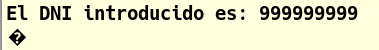
\includegraphics[width=0.5\textwidth]{mainmatter/Fotos Codigo/imagenimagem.png}

\chapter{SOLUCIONES}

\section{Soluciones generales}
\noindent Los desbordamientos de búfer representan una amenaza seria en el desarrollo de software, especialmente en lenguajes de bajo nivel como C, que no realiza verificaciones automáticas de los límites de la memoria. 
\\
A continuación, se presentan una serie de prácticas y herramientas que se utilizan ampliamente para prevenir y gestionar eficazmente los desbordamientos de búfer:

\begin{enumerate}
    \item \textbf{Uso de Funciones de Manipulación de Cadenas Seguras}
    \\
    Las funciones de manipulación de cadenas en C, como \verb|strcpy|, \verb|sprintf|, y \verb|strcat|, son conocidas por su vulnerabilidad a desbordamientos de búfer, ya que no tienen en cuenta los límites de la memoria asignada para las cadenas destino. Para minimizar el riesgo de desbordamiento de búfer y mejorar la seguridad del código, es fundamental adoptar funciones seguras que permitan controlar la cantidad de datos que se copian o concatenan en cada operación. Funciones como \verb|strncpy| y \verb|snprintf|, que permiten especificar la longitud máxima de los datos a copiar o formatear, son alternativas más seguras que deberían ser preferidas siempre que sea posible. También existen bibliotecas modernas y funciones especializadas en manipulación de cadenas seguras que están diseñadas específicamente para reducir este riesgo.

    \item \textbf{Validación de la Longitud de las Entradas}
    \\
    Validar la longitud de las entradas antes de almacenarlas en búferes de tamaño fijo es una práctica esencial en el desarrollo seguro de software. Esto implica verificar que los datos ingresados por el usuario o provenientes de otras fuentes externas no excedan la capacidad del búfer, evitando así la sobrescritura de áreas de memoria adyacentes. Esta validación debe hacerse tanto en tiempo de compilación como en tiempo de ejecución para garantizar que el programa funcione correctamente bajo condiciones normales y ante entradas inesperadas. En algunos casos, es conveniente establecer límites de longitud fijos y claros en la especificación del programa para facilitar esta tarea.

    \item \textbf{Asignación Dinámica de Memoria (cuando es posible)}
    \\
    La asignación dinámica de memoria mediante funciones como \verb|malloc|, \verb|calloc|, y \verb|realloc| en C permite al programa ajustar el tamaño del búfer de acuerdo con la cantidad de datos que necesita manejar en tiempo de ejecución. Esto reduce el riesgo de desbordamientos de búfer, ya que el tamaño de la memoria puede aumentar según la demanda del programa, en lugar de depender de un tamaño estático. Sin embargo, es importante recordar que un uso incorrecto de la memoria dinámica puede introducir otros problemas de seguridad, como filtraciones de memoria (\textit{memory leaks}) o uso de memoria no inicializada. Para evitar esto, los desarrolladores deben asegurarse de liberar correctamente la memoria asignada con \verb|free| después de que ya no sea necesaria y de inicializar adecuadamente cualquier memoria asignada.

    \item \textbf{Control y Seguimiento del Uso de Memoria}
    \\
    Monitorear y controlar el uso de la memoria del programa es otra estrategia efectiva para prevenir desbordamientos de búfer. Existen herramientas de análisis y depuración de memoria, como \textit{Valgrind}, que permite detectar posibles errores de memoria, incluyendo accesos fuera de los límites del búfer y uso de memoria sin inicializar. Estas herramientas pueden integrarse en el flujo de trabajo de desarrollo y ejecutarse durante pruebas exhaustivas para detectar y corregir vulnerabilidades antes de la fase de producción. Además, muchas herramientas de análisis de memoria proporcionan información detallada sobre el estado del programa, lo que permite identificar fácilmente áreas del código propensas a desbordamientos de búfer.

    \item \textbf{Desarrollo Seguro y Prácticas de Programación Defensiva}
    \\
    Implementar prácticas de programación defensiva y seguir principios de desarrollo seguro es fundamental para reducir el riesgo de desbordamiento de búfer y otros errores de seguridad. Esto incluye escribir código robusto que prevea posibles condiciones de error y situaciones de uso inesperadas, de modo que el programa responda de manera controlada y segura. La programación defensiva también implica una revisión constante del código para verificar que no existan accesos indebidos a la memoria y que los límites de los búferes se respeten en todas las operaciones de lectura y escritura. Además, el uso de revisiones de código y auditorías de seguridad puede ayudar a identificar problemas de memoria y prácticas inseguras en el código, lo cual es una excelente práctica para reducir errores en etapas tempranas del desarrollo.

\end{enumerate}


\section{Solución específica}
\noindent Para solucionar el buffer overflow en este programa, tendremos en cuenta los fallos que se han cometido hasta ahora:

\begin{enumerate}
    \item \textbf{No tener en cuenta el caracter nulo.}
    \item \textbf{Uso de función de copia de string insegura}\textbf{, no se controla el máximo de lectura}

\end{enumerate}
\noindent \textbf{1.} Vamos a modificar el código de tal forma que qfoo tenga espacio para 9 + 1 caracteres, incluyendo así el caracter nulo.
\begin{verbatim}
int
main ()
{
  char qfoo[9+1]; //Incluyendo caracter nulo
  char q0[9+1]; //Incluyendo caracter nulo
  int qbar = 0;
  char qbaz;
\end{verbatim}
\newpage \noindent
\textbf{2.} Ahora vamos a modificar el bucle while donde se lee de tal forma que no se pueda escribir más de lo que se debería en qfoo.
\begin{verbatim}
#include <stdio.h>
#include <string.h>
int
main ()
{
  char qfoo[9+1]; //Incluyendo caracter nulo
  char q0[9+1]; //Incluyendo caracter nulo
  int qbar = 0;
  char qbaz;
  printf
    ("Introduce el DNI caracter a caracter y presiona 
    Enter para terminar):\n");
  while ((qbaz = getchar ()) != '\n' && qbar<9) //Para que no 
  //se escriba más de 9 caracteres de DNI
    {
      qfoo[qbar++] = qbaz;
    }
  qfoo[qbar] = '\0';
  strcpy (q0, qfoo);
  printf ("El DNI introducido es: %s\n", q0);
  return 0;
}
\end{verbatim}

\noindent Por úiltimo vamos a pasarle valgrind para ver si se encuentra algún error.
Introduce el DNI caracter a caracter y presiona Enter para terminar): 
\\
999999999999999999999999999999999999999999999999999 
\\
El DNI introducido es: 999999999 
\\
==4366== HEAP SUMMARY: 
\\
==4366==     in use at exit: 0 bytes in 0 blocks 
\\
==4366==   total heap usage: 2 allocs, 2 frees, 2,048 bytes allocated 
\\
==4366==  
\\
==4366== All heap blocks were freed -- no leaks are possible 
\\
==4366==  
\\
\textbf{==4366== ERROR SUMMARY: 0 errors from 0 contexts (suppressed: 0 from 0)}
\\
Podemos observar que \textbf{no ocurre ningún error} ahora tras escribir de más.

\afterpage{\blankpage}

                          
 


\printbibliography

\end{document}